\tikzstyle{input_neuron}=[circle,draw=red!50,fill=orange!10,thick,minimum size=.2mm]
\tikzstyle{hidden_neuron}=[circle,draw=blue!50,fill=blue!10,thick,minimum size=1mm]
\tikzstyle{output_neuron}=[circle,draw=green!50,fill=green!20,thick,minimum size=1mm]
\tikzstyle{input}=[circle,draw=black!50,fill=black!20,thick,minimum size=.2mm]

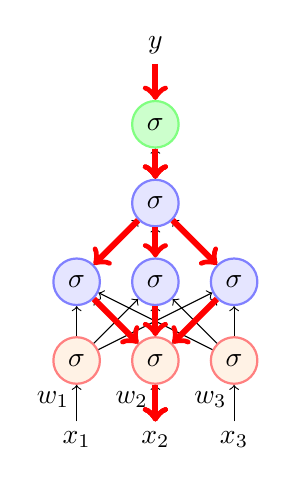
\begin{tikzpicture}

	\node [output_neuron] (out0) at (5,7)  {$\sigma$} ;
	
	\node [input_neuron] (in0) at (4,4)  {$\sigma$} ;
	\node (input0) at (4,3)  {$x_1$};
	\node [input_neuron] (in1) at (5,4)  {$\sigma$};
	\node [input_neuron] (in2) at (6,4)  {$\sigma$} ;
	\node (input1)  at (5,3) {$x_2$};
	\node (input2)  at (6,3) {$x_3$};
	
	\node [hidden_neuron] (hi0) at (4,5)  {$\sigma$} ;
	\node [hidden_neuron] (hi1) at (5,5)  {$\sigma$};
	\node [hidden_neuron] (hi2) at (6,5)  {$\sigma$} ;
	
	%\node [hidden_neuron] (hi3) at (4,6)  {$\sigma$} ;
	\node [hidden_neuron] (hi4) at (5,6)  {$\sigma$};
	%\node [hidden_neuron] (hi5) at (6,6)  {$\sigma$} ;
	
	\node (output0) (output0) at (5,8)  {$y$} ;
	
	
	\draw [->] (input0) -- (in0);
	\draw [->](input1) -- (in1);
	\draw [->] (input2) -- (in2);
	\draw [->] (in0) -- (hi0);
	\draw [->] (in0) -- (hi1);
	\draw [->] (in0) -- (hi2);
	\draw [->](in1) -- (hi0);
	\draw [->](in1) -- (hi1);
	\draw [->](in1) -- (hi2);
	\draw [->] (in2) -- (hi0);
	\draw [->] (in2) -- (hi1);
	\draw [->] (in2) -- (hi2);
	
	%\draw [->](hi0) -- (hi3);
	\draw [->](hi0) -- (hi4);
	%\draw [->](hi0) -- (hi5);
	%\draw [->](hi1) -- (hi3);
	\draw [->](hi1) -- (hi4);
	%\draw [->] (hi1) -- (hi5);
	%\draw [->] (hi2) -- (hi3);
	\draw [->] (hi2) -- (hi4);
	%\draw [->] (hi2) -- (hi5);
	
	\draw [->] (hi4) -- (out0);
	%\draw [->] (hi3) -- (out0);
	%\draw [->] (hi5) -- (out0);
	
	
	%\draw [->] (out0) -- (output0);
	\draw [->][line width=0.75mm,red] (output0) -- (out0);
	
	\node (formula) at (3.7,3.5) {$w_{1}$};
	\node (formula) at (4.7,3.5) {$w_{2}$};
	\node (formula) at (5.7,3.5) {$w_{3}$};
	
	
	\draw[line width=0.75mm,red] [->](hi4) -- (hi0);
	\draw[line width=0.75mm,red] [->](in1) -- (input1);
	\draw[line width=0.75mm,red] [->](hi0) -- (in1);
	\draw[line width=0.75mm,red] [->](out0) -- (hi4);
	
	
	\draw[line width=0.75mm,red] [->](hi4) -- (hi1);
	\draw[line width=0.75mm,red] [->](in1) -- (input1);
	\draw[line width=0.75mm,red] [->](hi1) -- (in1);
	\draw[line width=0.75mm,red] [->](out0) -- (hi4);
	
	\draw[line width=0.75mm,red] [->](hi4) -- (hi2);
	\draw[line width=0.75mm,red] [->](in1) -- (input1);
	\draw[line width=0.75mm,red] [->](hi2) -- (in1);
	\draw[line width=0.75mm,red] [->](out0) -- (hi4);
	%\draw (6.5,7) -- (7.5,7);
	%\draw (6.5,6) -- (7.5,6);
	%\draw (6.5,5) -- (7.5,5);
	
\end{tikzpicture}